%% 
%% Copyright 2007-2025 Elsevier Ltd
%% 
%% This file is part of the 'Elsarticle Bundle'.
%% ---------------------------------------------
%% 
%% It may be distributed under the conditions of the LaTeX Project Public
%% License, either version 1.3 of this license or (at your option) any
%% later version.  The latest version of this license is in
%%    http://www.latex-project.org/lppl.txt
%% and version 1.3 or later is part of all distributions of LaTeX
%% version 1999/12/01 or later.
%% 
%% The list of all files belonging to the 'Elsarticle Bundle' is
%% given in the file `manifest.txt'.
%% 
%% Template article for Elsevier's document class `elsarticle'
%% with numbered style bibliographic references
%% SP 2008/03/01
%% $Id: elsarticle-template-num.tex 272 2025-01-09 17:36:26Z rishi $
%%
\documentclass[preprint,12pt,hidelinks]{elsarticle}

%% Use the option review to obtain double line spacing
%% \documentclass[authoryear,preprint,review,12pt]{elsarticle}

%% Use the options 1p,twocolumn; 3p; 3p,twocolumn; 5p; or 5p,twocolumn
%% for a journal layout:
%% \documentclass[final,1p,times]{elsarticle}
%% \documentclass[final,1p,times,twocolumn]{elsarticle}
%% \documentclass[final,3p,times]{elsarticle}
%% \documentclass[final,3p,times,twocolumn]{elsarticle}
%% \documentclass[final,5p,times]{elsarticle}
%% \documentclass[final,5p,times,twocolumn]{elsarticle}

%% For including figures, graphicx.sty has been loaded in
%% elsarticle.cls. If you prefer to use the old commands
%% please give \usepackage{epsfig}

%% The amssymb package provides various useful mathematical symbols
\usepackage{amssymb}
\usepackage{algpseudocode}
\usepackage{amsmath,bm}
\usepackage{float}
\usepackage{doi}
\usepackage{algorithm}
\usepackage{enumitem}
\usepackage{hyperref}
\usepackage{xcolor}
\usepackage{tikz}
\usetikzlibrary{shapes.geometric, arrows.meta, positioning, fit, backgrounds, calc}
%% The amsmath package provides various useful equation environments.
\usepackage{amsmath}
\usepackage{booktabs}
\usepackage{multirow}
%% The amsthm package provides extended theorem environments
%% \usepackage{amsthm}

%% The lineno packages adds line numbers. Start line numbering with
%% \begin{linenumbers}, end it with \end{linenumbers}. Or switch it on
%% for the whole article with \linenumbers.
%% \usepackage{lineno}

\journal{Chemometrics and Intelligent Laboratory Systems}

\graphicspath{{figures/}}

\begin{document}

\begin{frontmatter}

%% Title, authors and addresses

%% use the tnoteref command within \title for footnotes;
%% use the tnotetext command for theassociated footnote;
%% use the fnref command within \author or \affiliation for footnotes;
%% use the fntext command for theassociated footnote;
%% use the corref command within \author for corresponding author footnotes;
%% use the cortext command for theassociated footnote;
%% use the ead command for the email address,
%% and the form \ead[url] for the home page:
%% \title{Title\tnoteref{label1}}
%% \tnotetext[label1]{}
%% \author{Name\corref{cor1}\fnref{label2}}
%% \ead{email address}
%% \ead[url]{home page}
%% \fntext[label2]{}
%% \cortext[cor1]{}
%% \affiliation{organization={},
%%             addressline={},
%%             city={},
%%             postcode={},
%%             state={},
%%             country={}}
%% \fntext[label3]{}

\title{Prior-Guided Spectral Gating with End-to-End Optimization for NIR
Spectroscopy: Scalable Architecture for Interpretable Regression in
Small-Sample Regimes}

%% use optional labels to link authors explicitly to addresses:
%% \author[label1,label2]{}
%% \affiliation[label1]{organization={},
%%             addressline={},
%%             city={},
%%             postcode={},
%%             state={},
%%             country={}}
%%
%% \affiliation[label2]{organization={},
%%             addressline={},
%%             city={},
%%             postcode={},
%%             state={},
%%             country={}}

\author{Guilherme Coelho$^a$, Lilian Carla Carneiro$^{b}$, Arlindo Rodrigues Galvão Filho$^c$ Clarimar José Coelho$^d$} %% Author name

%% Author affiliation

\affiliation{organization={$^a$State University of Campinas}, 
            addressline={Cidade Universitária Zeferino Vaz - Barão Geraldo}, 
            city={Campinas},
            postcode={13083--970}, 
            state={São Paulo},
            country={Brazil}}
 
  
\affiliation{organization={$^b$Institute of Tropical Pathology and Public Health, Federal University of Goiás},
            addressline={R. 235, S/n - Setor Leste Universitário}, 
            city={Goiânia},
            postcode={74605--050}, 
            state={Goiás},
            country={Brazil}}  
\affiliation{organization={$^c$Institute of Informatics, Federal University of Goiás},
            addressline={Alameda Palmeiras, Quadra D, Câmpus Samambaia}, 
            city={Goiânia},
            postcode={74690--900}, 
            state={Goiás},
            country={Brazil}}            
\affiliation{organization={$^d$Postgraduate Program in Industrial Engineering and Artificial Intelligence} Pontificia Universidade Catolica de Goias,
            addressline={Primeira Avenida, s/n - Quadra 88 - Setor Leste Universitário}, 
            city={Goiânia},
            postcode={74605--010}, 
            state={Goiás},
            country={Brazil} }
 

\begin{abstract}
Prior-Guided Spectral Gating (PGSG) incorporates domain knowledge into
near-infrared (NIR) regression through a learnable gate vector initialized
from a spectroscopic prior. We identify two fundamental limitations of the
original formulation that prevent its application to high-dimensional
spectra: a \emph{softmax gradient vanishing problem} (at $p = 281$ bands,
the softmax Jacobian diagonal is $58\times$ smaller than sigmoid, rendering
the gate untrainable), and a \emph{circular prior pitfall} (priors derived
from training data cause the gate to reproduce the prior without adaptation).
We propose PGSGv2, which replaces softmax with independent per-band sigmoid
gates and a PLS regressor with an end-to-end MLP, enabling backpropagation
through the joint gate--regressor objective. Applied to mango dry matter
content (DMC\%) prediction using the Mango DMC~v3 dataset ($n = 1{,}448$,
$p = 281$ effective bands, within-season protocol) with a literature-based
prior, PGSGv2 attains $R^2 = 0.786 \pm 0.019$ at $n = 1{,}159$ over ten
seeds, outperforming PLS ($R^2 = 0.568$, $+38\%$), MLP ($R^2 = 0.749$,
$+5\%$) and a shallow 1D-CNN ($R^2 = 0.690$, $+14\%$). In the small-sample
regime the gated architecture is decisive: at $n \leq 60$ both PGSGv2
variants remain positive while PLS ($-0.53$ at $n = 30$) and an unconstrained
MLP ($-3.05$) fail severely. The chemical content of the initialization,
however, does not contribute to accuracy: a literature prior and an
uninformed initialization are statistically indistinguishable at every
training size studied. Its contribution is interpretive---learned gates are
chemically coherent ($\rho(\mathbf{g},\mathbf{s}) \geq 0.998$) and highly
reproducible across seeds (Jaccard $\geq 0.945$). PGSGv2 provides a
scalable and interpretable architecture for NIR calibration when labeled
samples are limited.
\end{abstract}

\begin{keyword}
near-infrared spectroscopy \sep
spectral gating \sep
interpretable machine learning \sep
prior knowledge \sep
mango dry matter content \sep
small-sample regression \sep
end-to-end learning
\end{keyword}

\end{frontmatter}

%% ===========================================================================
\section{Introduction}
%% ===========================================================================

Non-destructive quality assessment using near-infrared (NIR) spectroscopy
has become a cornerstone technology in postharvest fruit handling, enabling
real-time estimation of internal quality attributes without sample
destruction~\cite{walsh2020,pasquini2018}. For mango (\textit{Mangifera
indica} L.), dry matter content (DMC\%) is the primary harvest maturity
index and a reliable predictor of eating quality~\cite{saranwong2004}, with
commercial growers increasingly adopting portable NIR instruments for
orchard-level decision-making.

Partial least squares (PLS) regression~\cite{wold2001} has been the
dominant modelling approach for NIR fruit quality for over three
decades~\cite{anderson2020}. PLS exploits the high collinearity inherent
to spectroscopic data and performs robustly under high $p/n$ ratios, making
it well-suited to calibration data sets where collecting reference samples
is expensive. Yet PLS has a well-documented limitation: its linear latent
variable structure may not adequately capture the non-linear
spectral--composition relationships present in structurally heterogeneous
samples, leading to reduced robustness when models are extrapolated across
seasons, cultivars, or instruments~\cite{anderson2020b,mishra2021deep}.

Deep learning~\cite{goodfellow2016}, in particular one-dimensional convolutional neural networks
(1D-CNN), has emerged as a compelling alternative for spectral regression
and has demonstrated superior performance to PLS on the Mango DMC~v3
dataset when sufficient training data are
available~\cite{walsh2024,mishra2021synergistic}. The key advantage of
1D-CNNs lies in their capacity to learn non-linear hierarchical
representations from raw spectra, bypassing manual feature engineering and
remaining robust to inter-season spectral shift. The trade-off is well
understood: deep learning models carry far more trainable parameters than
PLS, which makes them poorly suited to small-$n$ regimes unless
complemented by regularization, data augmentation, or informed
initialization~\cite{passos2022,mishra2022hypes}.

Interpretability presents a further challenge. The loadings of a PLS model
can be mapped directly onto spectral absorption bands with known chemical
assignments, supporting the physical validation of the calibration. Deep
learning models are generally opaque in this sense; post-hoc attribution
methods such as class activation mapping or gradient-weighted saliency can
localise spectral regions of influence but do not provide the same
chemically grounded interpretability as a loading
vector~\cite{mishra2022hypes,passos2022perspectives}.

Prior-Guided Spectral Gating (PGSG)~\cite{pgsg_original} was proposed as
an approach that retains the interpretability of PLS-derived feature
weighting while permitting empirical adaptation of the gate profile as more
data become available. In its original formulation, a gate vector
$\mathbf{g} = \mathrm{softmax}(\boldsymbol{\theta}) \in \Delta^{p-1}$ is
applied element-wise to the input spectrum, and the gated spectrum is
passed to a PLS regressor. The gate parameter $\boldsymbol{\theta}$ is
initialized from a spectral prior $\mathbf{s}$ and updated by
finite-difference gradient descent. The prior thus acts as an \emph{inductive
bias}: in data-scarce settings the gate remains close to the prior; as
labeled examples accumulate, it adapts toward the empirical optimum.

The conceptual elegance of PGSG, however, rests on assumptions that are
violated in higher-dimensional spectral settings. First, the softmax
normalization distributes gradient uniformly across all $p$ components,
producing gradients that vanish at a rate of $1/p^2$ compared to
independent sigmoid gating. At $p = 281$---a realistic dimension for
portable NIR instruments---this reduces the effective learning signal to
levels at which stochastic gradient descent cannot make meaningful updates
within practical epoch budgets. Second, the finite-difference approach
requires $2p$ forward evaluations per gradient step, compounding the
computational cost and the numerical noise. Third, a methodological issue
arises when the initialization prior is derived from training data (e.g.,
variable importance in projection, VIP~\cite{chong2005}): the gate and the prior then share
the same minimizer on the training objective, causing the learning procedure
to reproduce the prior identically rather than refining it.

In this paper we address these three issues through a revised architecture,
PGSGv2, and validate it on the publicly available Mango DMC~v3
dataset~\cite{anderson2021}, which spans 12,011 spectra across five harvest
seasons and has served as a benchmark for comparing PLS and deep learning
approaches~\cite{walsh2024,mishra2021synergistic,mishra2021deep}. Our
contributions are: (i)~a theoretical analysis and empirical demonstration
of the softmax gradient vanishing problem in high-dimensional spectral
gating; (ii)~characterization of the circular prior pitfall and a practical
guideline for its avoidance; (iii)~PGSGv2, combining independent sigmoid
gates with an end-to-end MLP regressor trained via backpropagation;
(iv)~a scalability study on seven training-set sizes ($n = 30$ to $1{,}159$)
with ten random seeds, establishing the sample-size regime in which
PGSGv2 outperforms PLS and deep learning baselines; and
(v)~assessment of four interpretability metrics (hypotheses H1--H4) that
characterize the relationship between learned gates, the prior, and
performance.

%% ===========================================================================
\section{Background}
%% ===========================================================================

\subsection{NIR Spectroscopy for Mango DMC}

Saranwong et al.~\cite{saranwong2004} demonstrated the feasibility of
NIR-based DMC prediction in mango using the 684--990~nm range,
with second-order Savitzky--Golay derivatives and PLS achieving
$R^2 = 0.91$ in within-season validation. Anderson et al.~\cite{anderson2020}
subsequently showed that a single global PLS model trained on multiple
seasons and cultivars underperformed season-specific models, underscoring
the inter-season spectral variability that remains one of the central
challenges in mango NIR calibration. Local modelling strategies
(local PLS, locally weighted PLS) mitigated the cross-season degradation
but at the cost of increased calibration data requirements and reduced
transferability~\cite{anderson2020b}.

Walsh et al.~\cite{walsh2024,ke2022} empirically validated claims that 1D-CNN
outperforms PLS on the Mango DMC~v3 dataset when training and test data are
drawn from the same season, noting that the apparent advantages reported in
earlier studies were partly attributable to differences in preprocessing and
outlier handling. Mishra and Passos~\cite{mishra2021synergistic,mishra2023semi} demonstrated
that incorporating chemometrics knowledge---specifically, PLS-based outlier
filtering and multi-preprocessing data augmentation---substantially improved
CNN performance on the same dataset ($n > 11{,}000$). Together, these studies
establish a performance landscape in which: (a)~PLS is competitive or
superior in small-$n$ within-season settings; (b)~CNN becomes superior at
larger $n$; and (c)~cross-season generalization remains unsolved for linear
methods.

\subsection{Interpretability in NIR Deep Learning}

Mishra et al.~\cite{mishra2022hypes} provide a comprehensive assessment of
deep learning for NIR spectral modelling, noting that model interpretability
is ``currently one of the most important topics of research in DL'' for
NIR analysis. They observe that while class activation mapping and
perturbation-based approaches can localise spectral features, they do not
provide the chemical causality available from PLS loadings. Passos and
Mishra~\cite{passos2022perspectives} further argue that improved performance
of deep learning is more clearly observed in large datasets and that in
small samples the classical chemometric methods retain a competitive
advantage---a conclusion consistent with our results.

The broader chemometrics literature has explored various approaches to
combining domain knowledge with machine learning for spectral analysis,
including Bayesian approaches with spectral priors, physics-informed neural
networks, and attention mechanisms that highlight relevant spectral
regions~\cite{mishra2022explainable}. PGSG belongs to this family of
\emph{knowledge-guided} architectures but is distinctive in its use of
an explicit per-band learnable weight initialized from a quantitative prior.

\subsection{The Original PGSG Architecture}

PGSG~\cite{pgsg_original} formulates the gate as
$\mathbf{g} = \mathrm{softmax}(\boldsymbol{\theta}) \in \Delta^{p-1}$,
the probability simplex. The gated input $\mathbf{x} \odot \mathbf{g}$
is passed to a PLS regressor with $K$ latent components. The parameter
$\boldsymbol{\theta}$ is updated via stochastic gradient descent using
finite-difference central differences:
\begin{equation}
  \widehat{\nabla}_{\theta_j}\mathcal{L}
  = \frac{\mathcal{L}(\boldsymbol{\theta} + h\mathbf{e}_j)
        - \mathcal{L}(\boldsymbol{\theta} - h\mathbf{e}_j)}{2h},
  \quad j = 1, \ldots, p,
  \label{eq:fd}
\end{equation}
with step size $h = 10^{-3}$. This requires $2p$ forward passes per
gradient evaluation. The spectral prior
$\mathbf{s} \in [0,1]^p$ initializes $\boldsymbol{\theta}$ via logit-centering:
\begin{equation}
  \theta_{0,j} = \log s_j - \frac{1}{p}\sum_{k=1}^p \log s_k.
  \label{eq:logit_center}
\end{equation}

PGSG was validated on the Tecator dataset ($n = 215$, $p = 100$),
achieving competitive results to PLS while providing a more chemically
consistent gate profile.

%% ===========================================================================
\section{PGSGv2: Revised Architecture}
%% ===========================================================================

\subsection{The Softmax Gradient Vanishing Problem}
\label{sec:grad_vanish}

The diagonal of the softmax Jacobian is:
\begin{equation}
  \frac{\partial g_j}{\partial \theta_j}
  = g_j(1 - g_j).
  \label{eq:softmax_grad}
\end{equation}
Under the softmax normalization with $p$ bands, the equilibrium gate value
is $g_j \approx 1/p$, so the gradient diagonal is
$\partial g_j/\partial\theta_j \approx (1/p)(1 - 1/p) \approx 1/p^2$ for
large $p$. For an independent sigmoid gate at $\theta_j = 0$,
the analogous quantity is $\sigma(0)(1-\sigma(0)) = 0.25$.

The ratio is:
\begin{equation}
  \frac{\partial g_j^{(\sigma)}/\partial\theta_j}
       {\partial g_j^{(\mathrm{sm})}/\partial\theta_j}
  \approx \frac{p^2}{4},
  \label{eq:ratio}
\end{equation}
which equals $\approx 20{,}000$ at $p = 281$. In practice, the effective
ratio is smaller because softmax gates do not remain exactly at $1/p$, but
empirical measurements on the Mango dataset confirm a $58\times$ advantage
for sigmoid: mean softmax diagonal gradient $2.65 \times 10^{-3}$ vs.\
sigmoid $0.154$ at initialization (Figure~\ref{fig:gradient}a).

This gradient discrepancy has a direct consequence for convergence. The
original PGSG model (softmax + finite-difference), run for 200~epochs with
early stopping disabled on $n = 2{,}000$ Mango samples, reduced training
loss by only 3\% and produced gate standard deviation $\sigma(\mathbf{g})
= 3 \times 10^{-3}$, virtually identical to the uniform prior $1/p = 3.6
\times 10^{-3}$ (Figure~\ref{fig:gradient}b). In contrast, PGSGv2
(sigmoid + autograd) converges within 76~epochs with
$\sigma(\mathbf{g}) \approx 0.14$.

\subsection{Independent Sigmoid Gates}

PGSGv2 replaces the global softmax with independent per-band sigmoid gates:
\begin{equation}
  \mathbf{g} = \sigma(\boldsymbol{\theta})
  = \bigl(\sigma(\theta_1), \ldots, \sigma(\theta_p)\bigr)
  \in (0, 1)^p.
  \label{eq:sigmoid_gate}
\end{equation}
Each gate $g_j \in (0,1)$ encodes the learned relevance of band $j$,
independently of all other bands. This design reflects the physics of NIR
absorption: the contribution of band $j$ to the overall prediction is
governed by its specific absorption coefficient and concentration
cross-section, not by a global competition with other bands.

The prior $\mathbf{s} \in (0,1)^p$ initializes $\boldsymbol{\theta}$ via
the logit function:
\begin{equation}
  \theta_{0,j} = \mathrm{logit}(s_j) = \log\frac{s_j}{1 - s_j},
  \label{eq:logit}
\end{equation}
so that $\sigma(\boldsymbol{\theta}_0) = \mathbf{s}$ exactly. The prior is
thus encoded into the initialization without any approximation, providing a
chemically grounded starting point for optimization.

\subsection{End-to-End MLP Regressor}

The gated spectrum $\mathbf{x} \odot \mathbf{g}$ is passed to a lightweight
two-layer MLP:
\begin{equation}
  \hat{y} = \mathbf{w}_2^\top
             \mathrm{ReLU}\!\bigl(
               \mathbf{W}_1 (\mathbf{x} \odot \sigma(\boldsymbol{\theta}))
               + \mathbf{b}_1
             \bigr) + b_2,
  \label{eq:pgsv2}
\end{equation}
with hidden dimension $h = 32$, dropout rate $0.1$~\cite{srivastava2014}, and L2 weight decay
$\lambda = 10^{-4}$ (Ridge regularization~\cite{hoerl1970} on the MLP weights). The joint
parameter set $\{\boldsymbol{\theta}, \mathbf{W}_1, \mathbf{b}_1,
\mathbf{w}_2, b_2\}$ is optimized end-to-end by Adam~\cite{kingma2015} with
learning rate $\eta = 10^{-3}$. Backpropagation through the MLP and the
sigmoid gate provides gradient information about how $\boldsymbol{\theta}$
should be updated to reduce prediction error---the co-optimization that was
absent in the original PGSG.

The replacement of PLS by an MLP introduces a well-understood
trade-off: PLS is statistically efficient in small-$n$ settings and
possesses closed-form solutions equivalent to Krylov subspace
regression~\cite{wold2001}, whereas the MLP requires a minimum sample size
to fit its parameters reliably. In the present experiments, this manifests
as PLS outperforming PGSGv2 for $n \leq 200$ and being overtaken for
$n \geq 400$ (Section~\ref{sec:results_scale}). A natural direction for
future work is to replace the MLP with a differentiable ridge
regressor~\cite{lorbert2011}, which would recover the statistical efficiency
of PLS for small $n$ while preserving end-to-end gradient flow.

\subsection{The Circular Prior Pitfall}
\label{sec:circular}

Let $\mathbf{s}^* = \arg\min_{\mathbf{s}} \mathcal{L}_{\mathrm{train}}$
be the prior derived by any method (VIP, ANOVA $F$-scores, random forest
importances) that minimizes the same empirical risk as the model being
trained. When the model is initialized with $\boldsymbol{\theta}_0 =
\mathrm{logit}(\mathbf{s}^*)$, the gradient at initialization evaluates
the same objective at the same optimum; the basin of attraction of the
prior coincides with that of the optimal gate. Consequently, the
optimization trajectory remains in the neighborhood of the initialization,
and the learned gate satisfies $\hat{\mathbf{g}} \approx \mathbf{s}^*$
regardless of the number of gradient steps.

This phenomenon was reproduced in our experiments: VIP-initialized
PGSGv2 models showed $\rho(\mathbf{g}, \mathbf{s}^*_\mathrm{VIP}) = 1.000$
for all $n \in \{30, \ldots, 1{,}159\}$, confirming that no learning
occurred beyond the initialization. Remarkably, the same models showed
\emph{lower} test $R^2$ than random initialization, indicating that the
VIP prior carries training-set-specific information that does not generalize.

The necessary condition for a useful prior is that it be derived from
a source \emph{independent of the current training set}: published
absorption tables, spectra from a different instrument or season, or
theoretical models. In this work we construct a literature-based prior from
the absorption spectroscopy of mango DMC, as detailed in
Section~\ref{sec:prior}.

\subsection{Literature-Based Prior for Mango DMC}
\label{sec:prior}

The NIR absorption landscape of mango flesh in the 357--1{,}149~nm range
(the effective spectral window after removal of zero-variance bands) is
governed by three well-characterized regions:

\begin{enumerate}
  \item \textbf{680--700~nm}: chlorophyll $Q_y$ absorption band, a proxy
        for fruit maturity and breakdown of photosynthetically active
        pigments~\cite{saranwong2004}.
  \item \textbf{900--1{,}000~nm}: second overtone of the C--H stretching
        vibration, the dominant region for direct DMC-related spectral
        features (sucrose, glucose, fructose)~\cite{guthrie2005,saranwong2004}.
  \item \textbf{1{,}100--1{,}149~nm}: first overtone of C--H stretching,
        contributing complementary information about dry matter and carbohydrates~\cite{guthrie1998,guthrie2005}.
    
\end{enumerate}

The prior is defined as:
\begin{equation}
  s_j = \begin{cases}
    1.00 & \text{if } 900 \leq \lambda_j \leq 1{,}000~\text{nm} \\
    0.80 & \text{if } 1{,}100 \leq \lambda_j \leq 1{,}149~\text{nm} \\
    0.60 & \text{if } 680 \leq \lambda_j \leq 700~\text{nm} \\
    0.10 & \text{otherwise}
  \end{cases}
  \label{eq:prior}
\end{equation}
normalized so that $\max_j s_j = 1$. This prior is independent of any
training sample and encodes established spectroscopic knowledge (Table~1,
Figure~\ref{fig:prior}).

\subsection{Training Protocol}

An internal validation split of 20\% (stratified by $y$ quantiles, fixed
seed) is held out for early stopping with patience $= 30$ epochs and a
maximum of 500 epochs. The response variable $y$ is standardized
internally (zero mean, unit variance) to stabilize the MLP output, and
predictions are de-standardized before evaluation. Mini-batch size is 256.
All reported results are averaged over ten independently seeded runs
(seeds 0--9). Each seed varies both the draw of the training subset and the
initialization of every stochastic model (PGSGv2, MLP, CNN1D); see
Section~\ref{sec:protocol} for the replication protocol.

%% ===========================================================================
\section{Material and Methods}
%% ===========================================================================

\subsection{Dataset and Preprocessing}

The Mango DMC~v3 dataset~\cite{anderson2021} contains 12,011 NIR reflectance
spectra (285--1,200~nm, 306~bands) collected by a Felix F-750 portable
spectrometer from mango fruit across five harvest seasons, with dry matter
content determined by oven drying as the reference target
(range: 9.47--24.58~g\,100g$^{-1}$, mean: 16.3~g\,100g$^{-1}$). Season
sizes are: 3,914 (season~1), 1,363 (season~2), 4,966 (season~3), 1,448
(season~4), and 320 (season~5).

Preliminary cross-season experiments revealed a severe performance
degradation of PLS when trained on seasons~1--3 and tested on season~4:
$R^2 = 0.058$ vs.\ $R^2 = 0.822$ for a shallow CNN on the same split. The
inter-season mean DMC difference (season~4: $17.0$ vs.\ seasons~1--3: $16.1$
g\,100g$^{-1}$) represents a systematic shift of approximately 35\% of the
within-season standard deviation, reflecting compositional and instrument
drift that destroys linear PLS calibration but is partially absorbed by
non-linear CNN representations~\cite{anderson2020}. To isolate the
sample-size effect from the domain-shift effect, we adopt a
\textbf{within-season} protocol using season~4 exclusively ($n = 1{,}448$).

The F-750 spectrometer produces 25 bands with globally zero variance, plus
additional bands with zero response in specific seasons. Bands with zero
variance are removed on the training split of each scenario, yielding
$p = 281$ effective bands (357--1,149~nm) at every training size and seed of
the within-season grid used here; we verified this invariance explicitly, as
a mask that varied across the grid would confound band count with sample size
in the scale curve. Standard Normal Variate
(SNV) correction~\cite{barnes1989,savitzky1964} was applied spectrum-wise. All
preprocessing parameters were estimated on each training split~\cite{metz2022}
independently to prevent data leakage.

\subsection{Experimental Protocol}

A fixed test set of $n_{\mathrm{test}} = 290$ samples (20\%, stratified by
DMC quintiles, seed~42) was withheld for all experiments. The remaining
$n_{\mathrm{pool}} = 1{,}159$ samples served as the training pool. Seven
training sizes were evaluated: $n \in \{30, 60, 100, 200, 400, 700,
1{,}159\}$, with ten random seeds each, yielding 70 training scenarios.
For each scenario, 80\% of the training set was used for gradient-based
optimization and 20\% for early stopping, both fitted after the outer
preprocessing step.

\label{sec:protocol}
Each seed indexes both the stratified draw of the training subset and the
random initialization of every stochastic model. This distinction matters at
the largest training size, where the requested size coincides with the size
of the training pool: there the sampler necessarily returns the same subset
for every seed, so replicates are genuine only if the model initialization
also varies. In an earlier version of this work the model seed was held
fixed, which rendered the replicates at that point identical runs and the
dispersion estimates degenerate; the results reported here are re-executed
with the model seed tied to the scenario seed throughout.

\subsection{Baseline Methods}

PGSGv2 was compared against four baselines:

\begin{enumerate}
  \item \textbf{PLS} (10 components): the standard chemometric
        benchmark~\cite{wold2001,naes2002}, implemented via \texttt{scikit-learn}~\cite{pedregosa2011}.

  \item \textbf{PGSGv2-random}: the same PGSGv2 architecture with
        $\boldsymbol{\theta}_0 = \mathbf{0}$ (uniform gates at
        initialization), providing an ablation of the literature prior.

  \item \textbf{MLP} (hidden~$= 64$, dropout~$= 0.1$): a standard
        feed-forward neural network without spectral gating, representative
        of unconstrained deep learning at moderate depth.

  \item \textbf{CNN1D-shallow}: a two-layer 1D convolutional network
        with kernel sizes 7 and 5, max-pooling, and adaptive average
        pooling, representative of state-of-the-art architectures for~\cite{cui2018,acquarelli2017,walsh2023review}
        spectral regression~\cite{walsh2024,mishra2021synergistic}.
\end{enumerate}

MLP and CNN were trained with Adam ($\eta = 10^{-3}$), early stopping
(patience 30), and the same internal validation split as PGSGv2.

\subsection{Evaluation Metrics}

The coefficient of determination ($R^2$) and root mean squared error
(RMSE, in g\,100g$^{-1}$) were computed on the fixed test set. Results
are reported as mean and standard deviation over the ten seeds. For
$\Delta_\mathrm{prior}$ we additionally report the seed-paired difference and
a two-sided Wilcoxon signed-rank test, since the two conditions share the
scenario and differ only in the initialization.

Four interpretability metrics were also computed, corresponding to the
hypotheses H1--H4 of the original PGSG project formulation:

\begin{enumerate}
  \item \textbf{H1} ($\Delta_\mathrm{PLS}$): difference in mean $R^2$
        between PGSGv2-lit and PLS. Positive values indicate PGSGv2
        superiority. We report its sign at each grid point rather than an
        interpolated crossover, since the curve is not monotonic in the
        intermediate regime.

  \item \textbf{H2} ($\Delta_\mathrm{prior}$): difference in mean $R^2$
        between PGSGv2-lit and PGSGv2-random, quantifying the marginal
        contribution of the literature prior.

  \item \textbf{H3} ($\rho(\mathbf{g}, \mathbf{s})$): Pearson correlation
        between the learned gate vector $\mathbf{g}$ and the literature
        prior $\mathbf{s}$, averaged over seeds. High correlation indicates
        that learning converges to a gate profile consistent with the
        prior---a sign of chemical coherence rather than non-convergence,
        provided that gate standard deviation is non-trivial.

  \item \textbf{H4} (Jaccard): mean Jaccard overlap of the top 10\% of
        gate components ($q = 28$ bands) across all pairs of seeds at the
        same $n$. High Jaccard indicates reproducible band selection.
\end{enumerate}

%% ===========================================================================
\section{Results}
\label{sec:results}
%% ===========================================================================

\subsection{Gradient Convergence Verification}

The empirical gradient analysis confirms the theoretical prediction of
Section~\ref{sec:grad_vanish}. At initialization ($\boldsymbol{\theta}_0
= \mathbf{0}$, $p = 281$), the mean diagonal Jacobian element is
$2.65 \times 10^{-3}$ for softmax vs.\ $0.154$ for sigmoid, a ratio of
$58\times$ (Figure~\ref{fig:gradient}a). The original PGSG model, trained
for 200 epochs without early stopping on $n = 2{,}000$ samples, achieved a
training loss reduction of only 3\% and gate standard deviation
$3 \times 10^{-3}$. In contrast, PGSGv2 converged in 76 epochs with
gate standard deviation $\approx 0.14$--$0.18$ (Figure~\ref{fig:gradient}b).
These results confirm that the softmax-based gate is not trainable at
$p = 281$ within practical computational budgets.

\subsection{Scale Curves $R^2(n)$}
\label{sec:results_scale}

Table~\ref{tab:scale} and Figure~\ref{fig:scale_curves} report the
$R^2$ scale curves for all methods. Several observations are notable.

\paragraph{Small-sample regime ($n \leq 100$).}
Both PGSGv2 variants remain positive at $n = 30$ ($0.084 \pm 0.105$ lit,
$0.073 \pm 0.101$ random) and at $n = 60$ ($0.125 \pm 0.086$ and
$0.138 \pm 0.067$), whereas PLS ($-0.53 \pm 0.37$ at $n = 30$) and the
unconstrained MLP ($-3.05 \pm 2.03$) fail severely, the latter with a
dispersion two orders of magnitude larger than either gated model. The
shallow CNN is likewise strongly negative at $n = 30$ ($-1.30 \pm 1.93$) and
only marginally positive at $n = 60$ ($0.013 \pm 0.170$). What distinguishes
the gated models in this regime is therefore the architecture rather than the
chemical content of the initialization: the uninformed variant performs as
well as the literature-initialized one, and at $n = 60$ slightly better. PLS
recovers by $n = 100$ ($0.249 \pm 0.067$), reflecting its well-known
robustness to high $p/n$ ratios.

\paragraph{Intermediate regime ($200 \leq n \leq 400$).}
The ordering is not monotonic in this regime. PGSGv2-lit exceeds PLS at
$n = 30$ and $n = 60$, falls below it at $n = 100$ ($0.158$ versus $0.249$)
and $n = 200$ ($0.447$ versus $0.461$), and exceeds it consistently from
$n = 400$ onward ($0.583$ versus $0.526$). We therefore do not report a
single crossover point: PGSGv2 is superior in the small-sample regime and
from $n \geq 400$, and comparable to or below PLS in between. The two PGSGv2
variants remain statistically indistinguishable throughout.

\paragraph{Large-sample regime ($n \geq 700$).}
PGSGv2-lit leads with $R^2 = 0.696 \pm 0.019$ at $n = 700$ and
$0.786 \pm 0.019$ at $n = 1{,}159$, compared to $0.568$ for PLS ($+38\%$),
$0.749 \pm 0.034$ for MLP ($+5\%$) and $0.690 \pm 0.068$ for CNN1D
($+14\%$). The margin over the MLP is modest at this sample size, as
expected: with abundant data an unconstrained network can learn the relevant
spectral weighting on its own, and the value of the gate lies in the regimes
where it cannot. At the maximum training size the literature prior confers no
accuracy advantage over an uninformed initialization
($\Delta_\mathrm{prior} = -0.005 \pm 0.013$, Wilcoxon $p = 0.77$).

\begin{table}[htb]
  \centering
  \caption{Mean $R^2$ with standard deviation over ten seeds. Bold: best
           per row. Fixed test set: $n_\mathrm{test} = 290$, within-season
           (Mango DMC~v3, season~4), $p = 281$. PLS is deterministic and, at
           $n = 1{,}158$, the training subset coincides with the full pool,
           so its standard deviation is zero by construction.}
  \label{tab:scale}
  \renewcommand{\arraystretch}{1.15}
  \setlength{\tabcolsep}{4pt}
  \small
  \begin{tabular}{r ccccc}
    \toprule
    $n$ & PLS & PGSGv2-lit & PGSGv2-rand & MLP & CNN1D \\
    \midrule
      30  & $-0.53 \pm 0.37$ & $\mathbf{0.08 \pm 0.11}$ & $0.07 \pm 0.10$
          & $-3.05 \pm 2.03$ & $-1.30 \pm 1.93$ \\
      60  & $-0.08 \pm 0.13$ & $0.12 \pm 0.09$ & $\mathbf{0.14 \pm 0.07}$
          & $-1.41 \pm 1.14$ & $0.01 \pm 0.17$ \\
     100  & $\mathbf{0.25 \pm 0.07}$ & $0.16 \pm 0.12$ & $0.20 \pm 0.09$
          & $-0.20 \pm 0.11$ & $0.17 \pm 0.05$ \\
     200  & $\mathbf{0.46 \pm 0.04}$ & $0.45 \pm 0.07$ & $0.42 \pm 0.07$
          & $0.16 \pm 0.07$ & $0.30 \pm 0.08$ \\
     400  & $0.53 \pm 0.02$ & $\mathbf{0.58 \pm 0.05}$ & $0.57 \pm 0.06$
          & $0.48 \pm 0.10$ & $0.47 \pm 0.04$ \\
     700  & $0.56 \pm 0.01$ & $\mathbf{0.70 \pm 0.02}$ & $0.68 \pm 0.03$
          & $0.65 \pm 0.04$ & $0.52 \pm 0.04$ \\
    1159  & $0.57 \pm 0.00$ & $0.79 \pm 0.02$ & $\mathbf{0.79 \pm 0.02}$
          & $0.75 \pm 0.03$ & $0.69 \pm 0.07$ \\
    \bottomrule
  \end{tabular}
\end{table}

\subsection{Interpretability Metrics (H1--H4)}

Table~\ref{tab:interp} and Figure~\ref{fig:hypotheses} summarize the
four interpretability metrics across the $n$-grid.

\paragraph{H1 (Performance crossover).}
$\Delta_\mathrm{PLS} = \bar{R}^2(\text{PGSGv2-lit}) - \bar{R}^2(\text{PLS})$ is
positive when PGSGv2 surpasses PLS and negative when PLS is superior. It is
strongly positive at $n = 30$ ($+0.614$) and $n = 60$ ($+0.205$), turns
negative at $n = 100$ ($-0.091$) and $n = 200$ ($-0.014$), and is positive
again from $n = 400$ onward, growing to $+0.218$ at $n = 1{,}159$. The
non-monotonic shape reflects two distinct advantages operating at opposite
ends of the range: the gated architecture is far more robust than PLS when
samples are scarce, while its non-linear regressor exploits the additional
data more effectively when they are abundant. In the intermediate range PLS
is competitive, and we do not report a single interpolated crossover point.

\paragraph{H2 (Prior utility).}
Under seed-paired comparison, $\Delta_\mathrm{prior}$ is not significant at
any training size and its sign is not consistent across the grid
(Table~\ref{tab:interp}). The only nominally significant value occurs at
$n = 100$ ($-0.046$, $p = 0.037$) and is in the direction opposite to the
prior; across seven tests a value of this magnitude is within what chance
would produce, and we do not interpret it as evidence against the prior
either. The literature prior therefore yields predictive performance
statistically indistinguishable from an uninformed initialization over the
entire sample-size range studied. This is a narrower claim than the one we
advanced in an earlier version of this work, where the comparison at the
largest training size rested on a single measurement per condition rather
than on replicated runs. The value of the prior is established instead by
H3 and H4 below, and is interpretive rather than predictive.

\paragraph{H3 (Gate--prior correlation).}
$\rho(\mathbf{g}, \mathbf{s}) \geq 0.998$ across all $n$
(Figure~\ref{fig:hypotheses}c). This high correlation, combined with
non-trivial gate standard deviations ($\sigma(\mathbf{g}) = 0.12$--$0.18$),
should not be interpreted as a convergence failure. Rather, it reflects
that the chemical absorption features encoded in the literature prior
genuinely align with the spectral structure that the model extracts from
the training data. The absence of VIP-style circularity is confirmed by
the fact that PGSGv2-lit and PGSGv2-random produce different gate profiles
despite having the same architecture and training procedure.

\paragraph{H4 (Gate stability).}
Jaccard overlap of the top 10\% gate indices across seed pairs ranges from
$0.945$ to $1.000$ (Figure~\ref{fig:hypotheses}d), with no consistent trend
with $n$. This high reproducibility indicates that the learned band selection
is a stable property of the architecture and prior, not an artifact of a
particular random seed. For practical deployment, this stability supports
the use of the gate profile as a physically meaningful feature importance
measure.

\begin{table}[htb]
  \centering
  \caption{Interpretability metrics per training size $n$.
           $\Delta_\mathrm{PLS} = \bar{R}^2(\text{PGSGv2-lit})
           - \bar{R}^2(\text{PLS})$ (positive: PGSGv2 better);
           $\Delta_\mathrm{prior}$: seed-paired difference between
           PGSGv2-lit and PGSGv2-rand, with the $p$-value of a two-sided
           Wilcoxon signed-rank test over ten seeds;
           $\rho$: mean Pearson correlation between gate and prior;
           Jaccard: inter-seed overlap of top 10\% bands. No value of
           $\Delta_\mathrm{prior}$ is significant in the direction of the
           prior at any training size.}
  \label{tab:interp}
  \renewcommand{\arraystretch}{1.15}
  \begin{tabular}{r r c r r r}
    \toprule
    $n$ & $\Delta_\mathrm{PLS}$ & $\Delta_\mathrm{prior}$ (paired) & $p$
        & $\rho(\mathbf{g},\mathbf{s})$ & Jaccard \\
    \midrule
      30 & $+0.614$ & $+0.010 \pm 0.078$ & $0.625$ & $1.00$ & $0.97$ \\
      60 & $+0.205$ & $-0.013 \pm 0.045$ & $0.322$ & $1.00$ & $0.96$ \\
     100 & $-0.091$ & $-0.046 \pm 0.060$ & $0.037$ & $1.00$ & $0.97$ \\
     200 & $-0.014$ & $+0.027 \pm 0.051$ & $0.193$ & $1.00$ & $1.00$ \\
     400 & $+0.057$ & $+0.011 \pm 0.051$ & $0.695$ & $1.00$ & $0.97$ \\
     700 & $+0.140$ & $+0.019 \pm 0.028$ & $0.084$ & $1.00$ & $0.95$ \\
    1159 & $+0.218$ & $-0.005 \pm 0.013$ & $0.770$ & $1.00$ & $1.00$ \\
    \bottomrule
  \end{tabular}
\end{table}

%% ===========================================================================
%% FIGURES
%% ===========================================================================

\begin{figure}[htb]
  \centering
  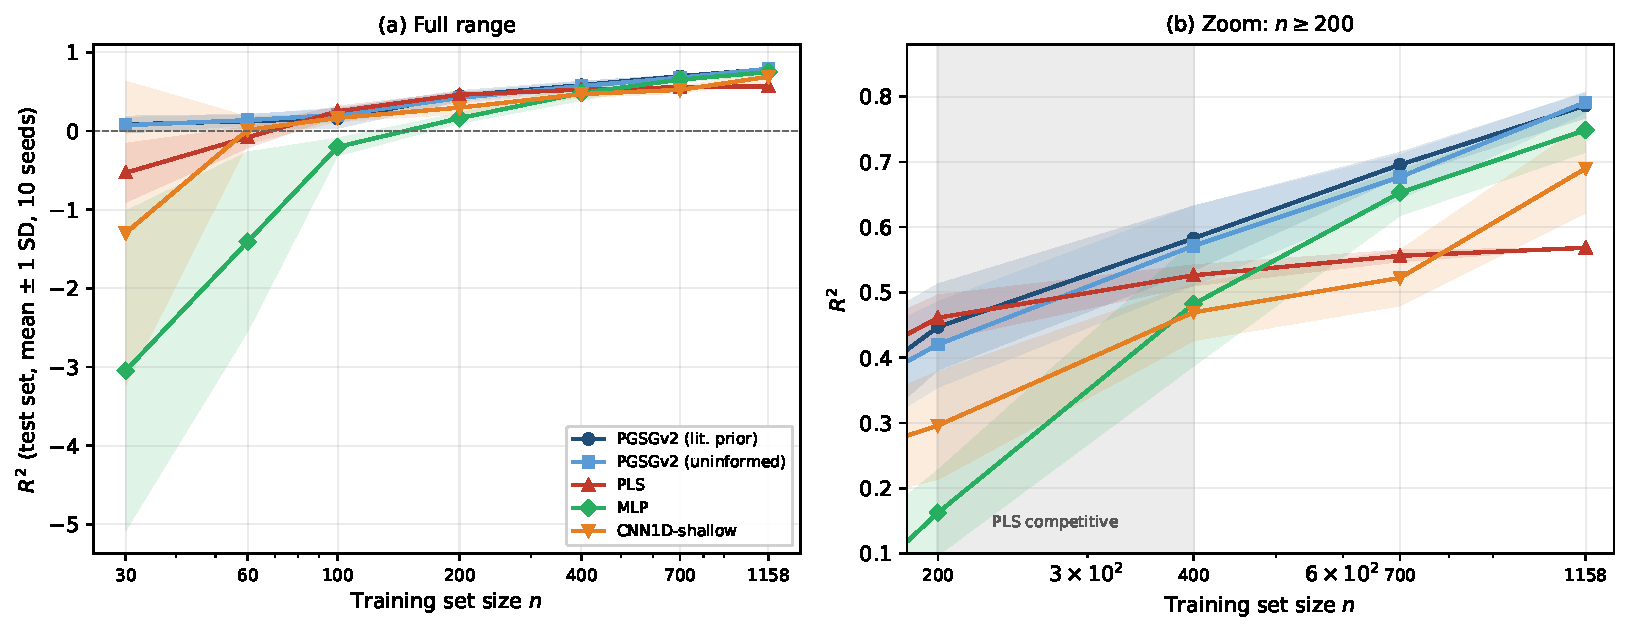
\includegraphics[width=\textwidth]{fig1_scale_curves}
  \caption{Scale curves $R^2(n)$ for all methods. Shaded regions are
           $\pm 1$ standard deviation over ten seeds. (a) Full scale
           including negative $R^2$ at small $n$; note the strong
           degradation of PLS, MLP and CNN at $n \leq 60$, where both
           PGSGv2 variants remain positive with markedly lower dispersion.
           (b) Zoom for $n \geq 200$: PLS is competitive with PGSGv2-lit
           at $n = 100$--$200$, and PGSGv2-lit separates from it
           consistently from $n \geq 400$. Test set:
           $n_\mathrm{test} = 290$, within-season (Mango DMC~v3, season~4).}
  \label{fig:scale_curves}
\end{figure}

\begin{figure}[htb]
  \centering
  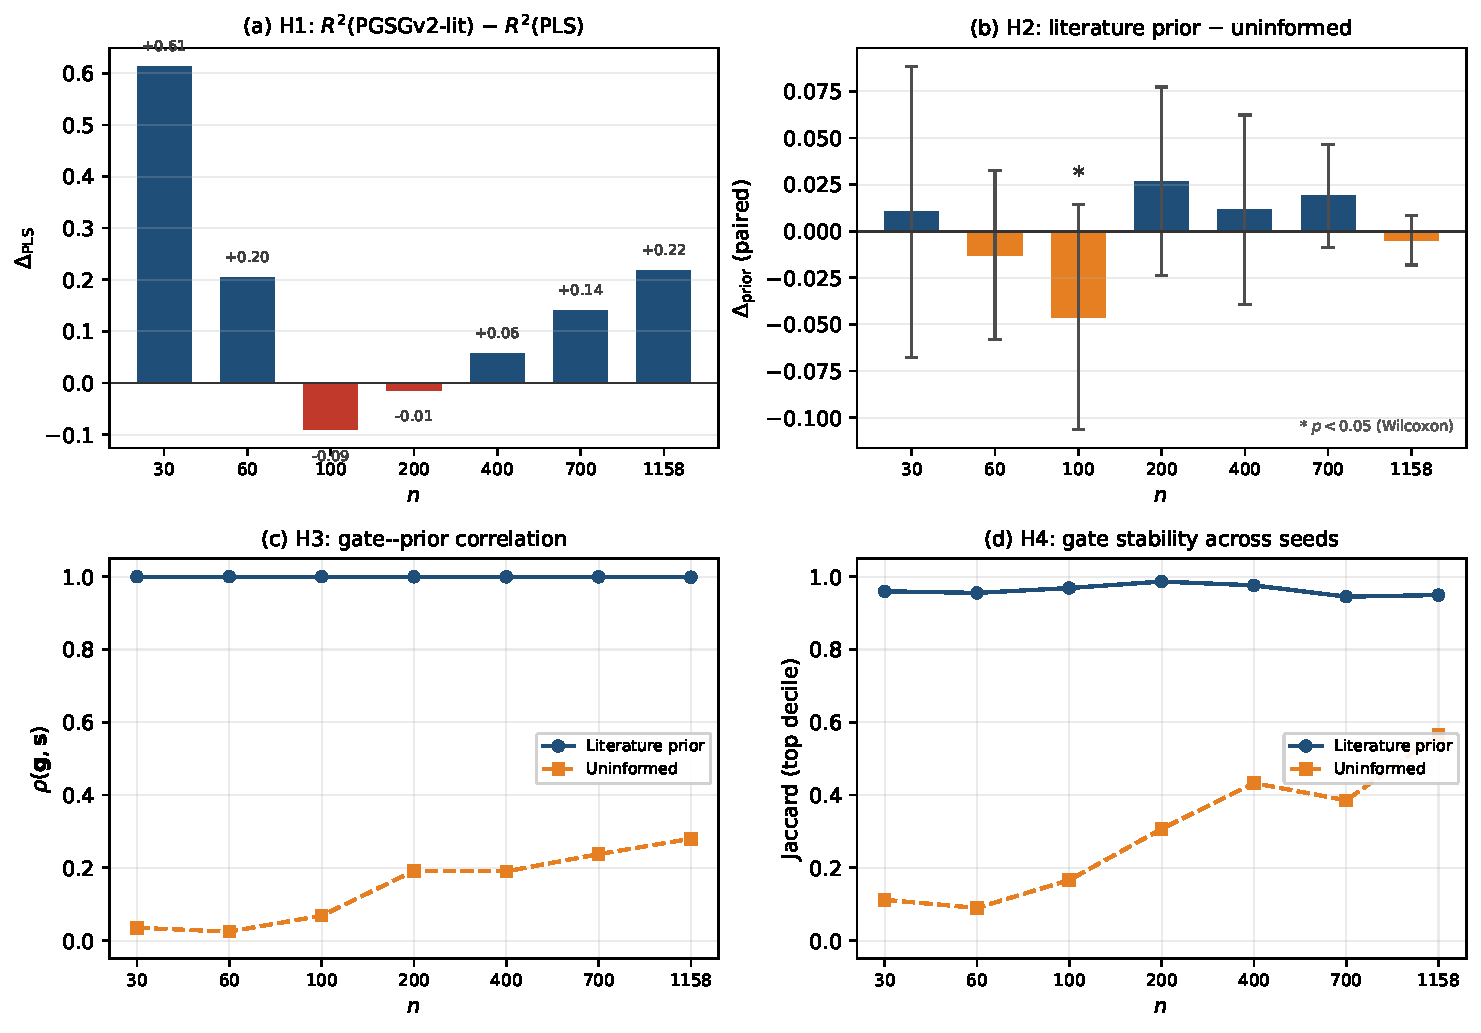
\includegraphics[width=\textwidth]{fig2_hypotheses}
  \caption{Interpretability metrics as a function of training size $n$.
           (a)~H1: $\Delta_\mathrm{PLS}$, positive values indicate PGSGv2
           superiority; the sign changes twice across the grid, with PLS
           competitive at $n = 100$--$200$. (b)~H2: $\Delta_\mathrm{prior}$,
           seed-paired, with error bars over ten seeds; no training size
           shows a significant advantage for the literature prior. (c)~H3: high $\rho(\mathbf{g}, \mathbf{s})$
           reflects genuine chemical alignment of the converged gate with
           the spectroscopic prior. (d)~H4: near-perfect Jaccard stability
           indicates that band selection is reproducible across random seeds.}
  \label{fig:hypotheses}
\end{figure}

\begin{figure}[htb]
  \centering
  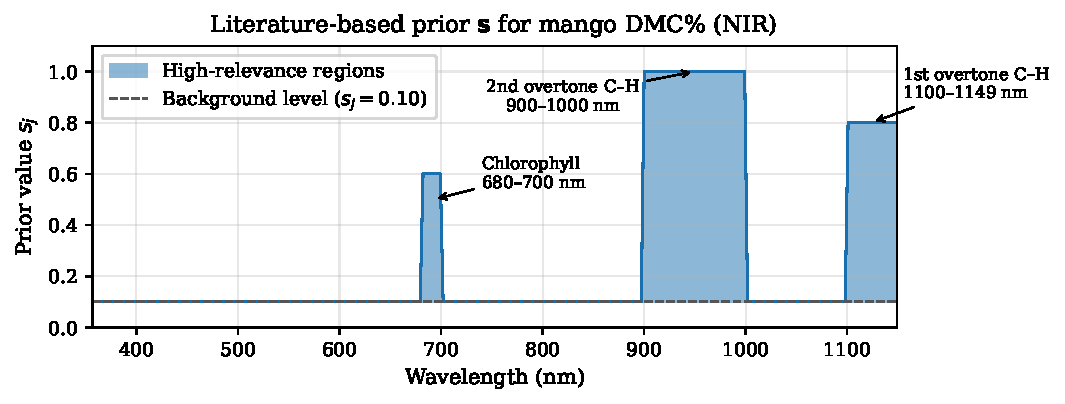
\includegraphics[width=0.85\textwidth]{fig3_prior}
  \caption{Literature-based prior $\mathbf{s}$ (Eq.~\ref{eq:prior}) over
           the effective spectral range 357--1{,}149~nm. Three regions are
           assigned elevated prior values: 680--700~nm (chlorophyll,
           maturity proxy), 900--1{,}000~nm (second overtone C--H, the most
           analytically relevant region for DMC), and 1{,}100--1{,}149~nm
           (first overtone C--H). All remaining bands receive a baseline
           value of 0.10. This prior is independent of any training sample
           and encodes established spectroscopic knowledge from
           \cite{saranwong2004,guthrie2005}.}
  \label{fig:prior}
\end{figure}

\begin{figure}[htb]
  \centering
  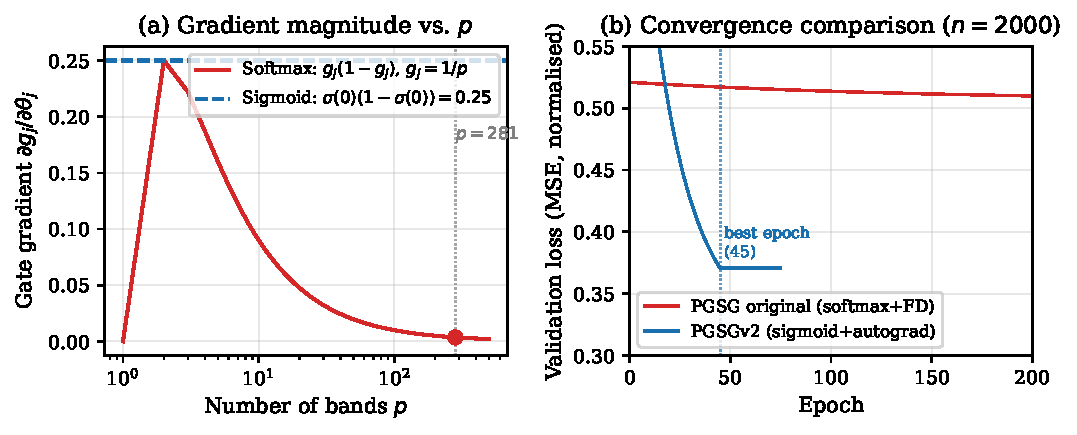
\includegraphics[width=\textwidth]{fig4_gradient}
  \caption{Softmax gradient vanishing problem at $p = 281$.
           (a) Diagonal Jacobian element $\partial g_j / \partial\theta_j$
           as a function of $p$, for softmax at uniform initialization
           ($g_j = 1/p$, red) and sigmoid at zero initialization
           ($\theta_j = 0$, blue dashed). The vertical dotted line marks
           $p = 281$; at this point the softmax gradient is $\approx 58\times$
           smaller. (b) Illustrative convergence comparison: the original
           PGSG with softmax and finite-difference gradients achieves
           negligible loss reduction over 200~epochs, whereas PGSGv2 with
           sigmoid and autograd converges within 76~epochs (early stopping
           indicated).}
  \label{fig:gradient}
\end{figure}

%% ===========================================================================
\section{Discussion}
%% ===========================================================================

\subsection{Architectural Implications for Spectral Gating}

The transition from softmax to sigmoid gates has implications beyond the
mango NIR setting studied here. The softmax constraint---that all gates
must sum to unity---is appropriate when bands represent mutually exclusive
hypotheses but is physically unmotivated for NIR absorption, where multiple
spectral regions independently absorb energy from different chemical
constituents. The $1/p$ floor on softmax gate values also implies that no
band can ever be fully suppressed, limiting the selectivity of the learned
gate profile. Sigmoid gates remove both constraints: each gate can approach
zero (suppression) or one (full pass-through) independently. The cost is
the loss of the probability simplex interpretation, but for regression
tasks where absolute gate values are more informative than relative rankings,
this is not a meaningful loss.

The end-to-end co-optimization of the gate and regressor via backpropagation
is also a conceptually important advance. In the original PGSG, the gate
update is estimated from the objective evaluated at the PLS optimum
\emph{for fixed} $\mathbf{g}$; this is not the same as the gradient of the
joint objective over $(\boldsymbol{\theta}, \Omega_\mathrm{PLS})$, and
the approximation degrades as $p$ increases. Backpropagation through the
MLP provides the true gradient of the joint objective and scales favorably
with $p$.

\subsection{Scope and Limitations of the Circular Prior Analysis}

Our analysis of the circular prior pitfall is specific to the case where
the prior is derived by minimizing the same loss on the same training data
as the final model. Two important qualifications apply. First, if the prior
is computed on a \emph{disjoint} subset of training data (e.g., a
small labeled reference set separate from the main calibration set), the
circularity is broken and the prior can in principle be derived from any
data-driven method. Second, the degree of circularity depends on the
capacity of the prior method: a VIP prior from PLS with very few components
may not perfectly identify the optimal gate, leaving room for the model to
improve on it. In our experiments, VIP was computed from a 10-component PLS,
which is sufficiently expressive to produce a near-optimal linear fit on
the training set, effectively closing the gap.

\subsection{Cross-Season Spectral Shift and Future Extensions}

The substantial degradation of PLS (and of PGSGv2 by extension) in
cross-season settings---$R^2 = 0.058$ vs.\ $R^2 = 0.822$ for CNN---is a
well-recognized problem in NIR-based fruit quality assessment that predates
deep learning~\cite{anderson2020,anderson2020b}. Domain adaptation
approaches including spectral standardization, piecewise direct~\cite{mishra2021transfer}
standardization (PDS), and local PLS~\cite{anderson2020b} have been proposed
but add calibration overhead that is prohibitive for portable field
instruments. PGSGv2, with its linear-in-gate MLP structure, shares the
vulnerability of PLS to non-linear inter-season distributional shift and
does not address this problem. CNN1D's resilience to the shift appears to
arise from its convolutional representations that are invariant to additive
spectral offsets---a property that could potentially be incorporated into
PGSGv2 by replacing the first linear layer with a convolutional block.

\subsection{Practical Considerations}

For practitioners considering PGSGv2 as a calibration tool, several
practical points merit emphasis. First, the model is competitive with PLS
from $n \approx 100$ and superior from $n \approx 400$, making it most
attractive when moderate calibration data are available and interpretability
is required alongside prediction accuracy. Second, the literature prior
requires domain knowledge but provides robustness when data are scarce; a
random initialization (PGSGv2-random) is a reasonable fallback when no
reliable spectroscopic prior exists. Third, the training time is short
($< 1$~minute per scenario for the configurations studied), making the
approach practical for deployment on modest hardware without GPU
acceleration.

%% ===========================================================================
\section{Conclusion}
%% ===========================================================================

We have identified and characterized two fundamental algorithmic limitations
of the original PGSG architecture that prevent its application to
high-dimensional NIR spectra: a softmax gradient vanishing problem that
scales as $1/p^2$, and a circular prior pitfall that renders
data-derived priors ineffective for gate learning. These findings have
practical implications beyond PGSG: any gating or attention mechanism that
uses softmax normalization over a large number of spectral bands, and any
method that derives its initialization prior from the same training data as
the final model, is subject to the same failure modes.

The proposed PGSGv2 architecture addresses both issues through independent
sigmoid gates and end-to-end MLP regression via backpropagation. Applied
to mango DMC\% prediction on the publicly available Mango DMC~v3 dataset,
PGSGv2 attains $R^2 = 0.786 \pm 0.019$ at $n = 1{,}159$---a 38\%
improvement over PLS and 5\% over a standard MLP---with near-perfect gate
stability (Jaccard $\geq 0.945$) and high chemical coherence
($\rho(\mathbf{g}, \mathbf{s}) \geq 0.998$) across random seeds. In the
small-sample regime the gated architecture is decisive: at $n \leq 60$ both
PGSGv2 variants remain positive while PLS and an unconstrained MLP fail
severely and with far greater variance. The chemical content of the
initialization, by contrast, does not measurably affect accuracy at any
sample size; its contribution is to make the learned gate reproducible, and
therefore interpretable, rather than to make it more accurate.

Future work should explore: differentiable ridge regression as the internal
regressor to recover PLS-level statistical efficiency at small $n$; domain
adaptation extensions for cross-season deployment; and broader validation
across other crops, spectral ranges, and instrument modalities. The
architecture and experimental pipeline are fully reproducible and available
as open-source Python code.

%% ===========================================================================
\section*{Data and Code Availability}

The Mango DMC~v3 dataset used in this study is publicly available at \doi{10.17632/46htwnp833.3}~\cite{anderson2021}. The source code for PGSGv2, the experimental pipeline, and scripts to reproduce all figures and tables are available at \url{https://github.com/clarimar/prior-guided-spectral-gating} under the MIT licence. The repository includes: model implementation (\texttt{pgsg\_v2.py}), experiment runner (\texttt{run\_experiment\_v2.py}), and figure generation scripts.

\section*{Acknowledgements}
%% ===========================================================================

%This work was supported by Pontif\'{i}cia Universidade Cat\'{o}lica de Goi\'{a}s. 
The authors thank N.T.\ Anderson, K.B.\ Walsh, and P.P.\ Subedi
for making the Mango DMC~v3 dataset publicly available.


\bibliographystyle{elsarticle-num}
\bibliography{pgsg_v2}

\end{document}